\documentclass[12pt,a4paper]{article}

\usepackage[a4paper,margin=2.4cm]{geometry}
\usepackage{amsmath,amssymb,bm}
\usepackage{siunitx}
\usepackage{booktabs}
\usepackage{array}
\usepackage{longtable}
\usepackage{graphicx}
\usepackage{hyperref}
\usepackage{xcolor}
\usepackage{float}
\usepackage{caption}

\hypersetup{
  colorlinks=true,
  linkcolor=blue!50!black,
  urlcolor=blue!50!black,
  citecolor=blue!50!black
}

\graphicspath{{outputs/}}
\setlength{\parskip}{0.45em}
\setlength{\parindent}{2em}

\title{Technical Documentation for the Rb87 Bias-Coil and 3D MOT Gradient-Field Simulation}
\author{MIGA Program}
\date{\today}

\begin{document}

\maketitle
\tableofcontents
\newpage

\section{Purpose of This Document}

This document describes the functionality, physical assumptions, and governing formulas of the simulation code centered on \texttt{rb87\_bias\_coils\_current\_scan.py}. The program is intended for Rb87 cold-atom experiments and focuses on the optical molasses / polarization-gradient-cooling (PGC) stage after the 3D MOT magnetic field is switched off.

The present version of the code is designed to answer the following practical questions:
\begin{itemize}
  \item How does the final molasses temperature depend on the compensation currents in the three bias-coil pairs?
  \item How does the answer change if the atomic cloud is not exactly located at the magnetic-field zero?
  \item How does the residual 3D MOT quadrupole field influence the compensation effectiveness when the cloud is displaced from the origin?
  \item How do the compensation coils modify not only the field at the cloud center, but also the local field profile around the cloud?
\end{itemize}

\section{Code Structure and Main Files}

\begin{longtable}{>{\raggedright\arraybackslash}p{0.34\textwidth} >{\raggedright\arraybackslash}p{0.58\textwidth}}
\toprule
File & Role \\
\midrule
\endhead
\texttt{rb87\_bias\_coils\_current\_scan.py} & Main simulation core. Contains coil-field calculation, MOT gradient-field calculation, temperature evolution, current scan, local refinement, plot generation, and summary export. \\
\texttt{rb87\_bias\_coils\_current\_scan\_ui.py} & Qt desktop interface for interactive parameter tuning and figure inspection. \\
\texttt{rb87\_bias\_coils\_current\_scan\_ui\_tk.py} & Tk fallback interface used when Qt is unavailable or unstable. \\
\texttt{example\_config.json} & Example configuration file containing atomic, molasses, bias-coil, MOT-gradient-coil, scan, and spatial-probe parameters. \\
\texttt{outputs/} & Output folder containing CSV tables, PNG figures, summary files, and resolved configuration files. \\
\bottomrule
\end{longtable}

\section{Coordinate System and Geometry}

\subsection{Atomic-Cloud Position}

The optical molasses stage is evaluated at the center of the atomic cloud,
\begin{equation}
  \bm{r}_0 = (x_0, y_0, z_0),
\end{equation}
with coordinates expressed in \si{mm}. In the configuration file this is written as
\begin{equation}
  \texttt{molasses\_position\_mm} = [x_0, y_0, z_0].
\end{equation}

By default,
\begin{equation}
  \bm{r}_0 = (0,0,0),
\end{equation}
which means that the cloud center coincides with the geometric center of the compensation-coil arrangement and the nominal zero of the MOT quadrupole field.

\subsection{Three-Axis Compensation Coil Pairs}

The compensation system consists of three square coil pairs aligned with the laboratory axes $X$, $Y$, and $Z$. Each axis is modeled as one symmetric pair of square loops:
\begin{itemize}
  \item each coil has $N_{\mathrm{comp}}$ turns,
  \item each loop has side length $L$,
  \item the two loop centers are placed at $\pm d_{\mathrm{comp}}$ along the corresponding axis,
  \item the two coils in one pair produce the same field direction near the center.
\end{itemize}

The current default geometry is
\begin{equation}
  N_{\mathrm{comp}} = 15,
  \qquad
  L = \SI{30}{cm},
  \qquad
  d_{\mathrm{comp}} = \SI{20}{cm}.
\end{equation}

\subsection{3D MOT Gradient-Coil Pair}

The simulation also contains a dedicated model for the 3D MOT magnetic coils. They are represented as a circular anti-Helmholtz pair:
\begin{itemize}
  \item each coil has $N_{\mathrm{MOT}}$ turns,
  \item each coil has radius $R_{\mathrm{MOT}}$,
  \item the two coil centers are located at $\pm d_{\mathrm{MOT}}$ along a chosen axis,
  \item the two coil currents have opposite sign, producing a near-zero field and non-zero gradient at the origin.
\end{itemize}

In the current example configuration,
\begin{equation}
  N_{\mathrm{MOT}} = 50,
  \qquad
  R_{\mathrm{MOT}} = \SI{10}{cm},
  \qquad
  d_{\mathrm{MOT}} = \SI{10}{cm},
  \qquad
  I_{\mathrm{MOT}} = \SI{7}{A}.
\end{equation}

The coil-pair axis is taken to be parallel to the line $y=z$, that is,
\begin{equation}
  \hat{\bm{u}}_{\mathrm{MOT}} \parallel (0,1,1).
\end{equation}
Internally the program normalizes this direction:
\begin{equation}
  \hat{\bm{u}}_{\mathrm{MOT}} =
  \frac{(u_x,u_y,u_z)}{\sqrt{u_x^2+u_y^2+u_z^2}},
\end{equation}
which for the default case becomes
\begin{equation}
  \hat{\bm{u}}_{\mathrm{MOT}} = \frac{(0,1,1)}{\sqrt{2}}.
\end{equation}

\section{Compensation-Coil Field Model}

\subsection{Biot--Savart Law}

The compensation-coil field is calculated from the Biot--Savart law,
\begin{equation}
  \bm{B}(\bm{r}) =
  \frac{\mu_0 I}{4\pi}
  \oint
  \frac{d\bm{\ell}' \times (\bm{r}-\bm{r}')}{|\bm{r}-\bm{r}'|^3}.
\end{equation}

Rather than using a purely on-axis center formula everywhere, the program discretizes each square loop into finite straight segments and evaluates the field numerically. This is important because once the cloud is displaced from the origin, off-diagonal coupling terms naturally appear.

\subsection{Current-to-Field Matrix}

At the cloud center $\bm{r}_0$, the compensation-coil contribution is written as
\begin{equation}
  \bm{B}_{\mathrm{comp}}(\bm{r}_0)
  =
  \bm{M}_{\mathrm{comp}}(\bm{r}_0)\,
  \bm{I}_{\mathrm{comp}},
\end{equation}
where
\begin{equation}
  \bm{I}_{\mathrm{comp}} =
  \begin{bmatrix}
    I_x \\ I_y \\ I_z
  \end{bmatrix},
\end{equation}
and
\begin{equation}
  \bm{M}_{\mathrm{comp}}(\bm{r}_0)
  =
  \begin{bmatrix}
    M_{xx} & M_{xy} & M_{xz} \\
    M_{yx} & M_{yy} & M_{yz} \\
    M_{zx} & M_{zy} & M_{zz}
  \end{bmatrix}.
\end{equation}

When $\bm{r}_0=(0,0,0)$ and the geometry is perfectly symmetric, the matrix is approximately diagonal:
\begin{equation}
  \bm{M}_{\mathrm{comp}}(0) \approx
  \begin{bmatrix}
    M_0 & 0 & 0 \\
    0 & M_0 & 0 \\
    0 & 0 & M_0
  \end{bmatrix}.
\end{equation}

For the current default geometry, the code yields approximately
\begin{equation}
  M_0 \approx \SI{296.35}{mG/A}.
\end{equation}

\section{3D MOT Gradient-Field Model}

\subsection{Anti-Helmholtz Circular Pair}

The 3D MOT field is modeled as the superposition of two circular coils with opposite currents. If the coil centers are
\begin{equation}
  \bm{r}_{\pm} = \pm d_{\mathrm{MOT}} \hat{\bm{u}}_{\mathrm{MOT}},
\end{equation}
then the field at position $\bm{r}$ is written as
\begin{equation}
  \bm{B}_{\mathrm{MOT}}(\bm{r})
  =
  \bm{B}_{\circ}\!\left(\bm{r}; \bm{r}_{+}, +I_{\mathrm{MOT}}\right)
  +
  \bm{B}_{\circ}\!\left(\bm{r}; \bm{r}_{-}, -I_{\mathrm{MOT}}\right),
\end{equation}
where $\bm{B}_{\circ}$ denotes the field from one circular loop.

Because the two currents have opposite sign, the origin is close to a magnetic-field zero:
\begin{equation}
  \bm{B}_{\mathrm{MOT}}(\bm{0}) \approx \bm{0},
\end{equation}
while the gradient is non-zero.

\subsection{Local Gradient Tensor}

The code also evaluates the local Jacobian of the MOT field near the cloud center,
\begin{equation}
  \bm{G}_{\mathrm{MOT}}(\bm{r}_0)
  =
  \nabla \bm{B}_{\mathrm{MOT}}(\bm{r}_0)
  =
  \begin{bmatrix}
    \dfrac{\partial B_x}{\partial x} &
    \dfrac{\partial B_x}{\partial y} &
    \dfrac{\partial B_x}{\partial z} \\
    \dfrac{\partial B_y}{\partial x} &
    \dfrac{\partial B_y}{\partial y} &
    \dfrac{\partial B_y}{\partial z} \\
    \dfrac{\partial B_z}{\partial x} &
    \dfrac{\partial B_z}{\partial y} &
    \dfrac{\partial B_z}{\partial z}
  \end{bmatrix}_{\bm{r}=\bm{r}_0}.
\end{equation}

Numerically, the derivatives are approximated using central differences:
\begin{equation}
  \frac{\partial \bm{B}}{\partial q}
  \approx
  \frac{\bm{B}(\bm{r}_0+\Delta q\,\hat{\bm{e}}_q)-\bm{B}(\bm{r}_0-\Delta q\,\hat{\bm{e}}_q)}{2\Delta q}.
\end{equation}

\section{Total Magnetic Field During Optical Molasses}

The total field at the cloud center during molasses is modeled as
\begin{equation}
  \bm{B}_{\mathrm{tot}}(t,\bm{r}_0)
  =
  \bm{B}_{\mathrm{stray}}
  +
  \bm{B}_{\mathrm{comp}}(\bm{r}_0)
  +
  e^{-t/\tau_{\mathrm{off}}}\,\bm{B}_{\mathrm{switch}}
  +
  e^{-t/\tau_{\mathrm{off}}}\,\bm{B}_{\mathrm{MOT,res}}(\bm{r}_0).
\end{equation}

Here:
\begin{itemize}
  \item $\bm{B}_{\mathrm{stray}}$ is the static background stray field,
  \item $\bm{B}_{\mathrm{comp}}(\bm{r}_0)$ is the compensation field at the cloud center,
  \item $\bm{B}_{\mathrm{switch}}$ is an empirical switch-off residual field,
  \item $\bm{B}_{\mathrm{MOT,res}}(\bm{r}_0)$ is the local residual field from the MOT gradient pair,
  \item $\tau_{\mathrm{off}}$ is the switch-off decay time constant.
\end{itemize}

The code introduces a configurable scale factor $s_{\mathrm{MOT}}$ for the MOT residual:
\begin{equation}
  \bm{B}_{\mathrm{MOT,res}}(\bm{r}_0) =
  s_{\mathrm{MOT}}\,\bm{B}_{\mathrm{MOT}}(\bm{r}_0).
\end{equation}

Therefore, if the atomic cloud is exactly at the magnetic zero, the MOT residual term can remain very small. If the cloud is displaced, however, the local quadrupole field becomes non-zero and can significantly alter the early molasses dynamics.

\section{Cooling-Efficiency Model}

\subsection{Magnetic Sensitivity}

The effective Zeeman sensitivity is written as
\begin{equation}
  \chi_B = |g_F|\,\frac{\mu_B}{h},
\end{equation}
converted in the code to units of \si{Hz/mG}.

\subsection{Optical Pumping Rate}

The total saturation parameter is taken as
\begin{equation}
  s_{\mathrm{tot}} = N_{\mathrm{beam}}\,s_0,
\end{equation}
where $s_0$ is the saturation parameter per beam and $N_{\mathrm{beam}}$ is the number of beams.

The optical pumping rate is approximated as
\begin{equation}
  \Gamma_{\mathrm{op}}
  =
  \frac{1}{2}\Gamma
  \frac{s_{\mathrm{tot}}}{1+s_{\mathrm{tot}}+4(\Delta/\Gamma)^2},
\end{equation}
where $\Gamma$ is the natural linewidth and $\Delta$ is the laser detuning.

\subsection{Effective Magnetic Width}

Unless manually overridden, the code defines an effective magnetic width
\begin{equation}
  B_{\mathrm{width}}
  =
  \alpha_{\mathrm{op}}
  \frac{\Gamma_{\mathrm{op}}}{\chi_B},
\end{equation}
where $\alpha_{\mathrm{op}}$ is the empirical width-scale factor corresponding to \texttt{optical\_pumping\_width\_scale}.

\subsection{Relative Cooling Efficiency}

The suppression of cooling by residual magnetic field is modeled as
\begin{equation}
  \eta_{\mathrm{raw}}(t)
  =
  \frac{1}{1+\left(\dfrac{|\bm{B}_{\mathrm{tot}}(t,\bm{r}_0)|}{B_{\mathrm{width}}}\right)^2}.
\end{equation}

The code then applies a lower clipping threshold:
\begin{equation}
  \eta(t)
  =
  \min\!\left(1,\max\!\left[\eta_{\min}, \eta_{\mathrm{raw}}(t)\right]\right).
\end{equation}

\section{Temperature-Evolution Model}

\subsection{Field-Dependent Equilibrium Temperature}

Let $T_0$ be the zero-field limit temperature and $T_{\mathrm{fail}}$ be the high-field failure temperature. The instantaneous equilibrium temperature is written as
\begin{equation}
  T_{\mathrm{eq}}(t)
  =
  T_0 + \left(T_{\mathrm{fail}}-T_0\right)\left[1-\eta_{\mathrm{raw}}(t)\right].
\end{equation}

Thus:
\begin{itemize}
  \item for $|\bm{B}| \to 0$, one has $\eta_{\mathrm{raw}} \to 1$ and therefore $T_{\mathrm{eq}} \to T_0$;
  \item for $|\bm{B}| \gg B_{\mathrm{width}}$, one has $\eta_{\mathrm{raw}} \to 0$ and therefore $T_{\mathrm{eq}} \to T_{\mathrm{fail}}$.
\end{itemize}

\subsection{Field-Dependent Cooling Time Constant}

If $\tau_0$ denotes the zero-field cooling time, the code defines
\begin{equation}
  \tau_{\mathrm{cool}}(t) = \frac{\tau_0}{\eta(t)}.
\end{equation}

\subsection{Temperature Dynamics}

The temperature follows
\begin{equation}
  \frac{dT}{dt}
  =
  -\frac{T(t)-T_{\mathrm{eq}}(t)}{\tau_{\mathrm{cool}}(t)}.
\end{equation}

The implementation uses explicit Euler stepping:
\begin{equation}
  T_{n+1}
  =
  T_n
  -
  \frac{T_n-T_{\mathrm{eq},n}}{\tau_{\mathrm{cool},n}}\,\Delta t.
\end{equation}

The final temperature $T_{\mathrm{final}}$ is the temperature at the end of the molasses time window.

\section{Current Scan and Local Refinement}

\subsection{Coarse Scan}

The simulation first evaluates a user-defined three-dimensional current grid,
\begin{equation}
  I_x \in [I_{x,\min}, I_{x,\max}],
  \quad
  I_y \in [I_{y,\min}, I_{y,\max}],
  \quad
  I_z \in [I_{z,\min}, I_{z,\max}].
\end{equation}

For every current triplet $(I_x,I_y,I_z)$, the code runs one full temperature-evolution simulation and stores:
\begin{itemize}
  \item the final temperature,
  \item the cooling efficiency,
  \item the compensation field at the cloud center,
  \item the mean, initial, and final residual-field magnitudes.
\end{itemize}

\subsection{Local Refinement}

If refinement is enabled, the code automatically narrows the scan window around the best coarse point and attempts to reach a target current step
\begin{equation}
  \Delta I_{\mathrm{target}}.
\end{equation}

This allows the workflow to preserve both:
\begin{itemize}
  \item a sufficiently broad coarse scan, and
  \item a fine final overview around the optimum.
\end{itemize}

\section{Local Spatial Field Curves}

In addition to the time evolution at the cloud center, the code evaluates one-dimensional field cuts around the cloud. For a probe direction $\hat{\bm{e}}$, the sampled positions are
\begin{equation}
  \bm{r}(s) = \bm{r}_0 + s\,\hat{\bm{e}},
\end{equation}
with
\begin{equation}
  s \in [-s_{\max}, s_{\max}],
\end{equation}
where $s_{\max}$ is controlled by the \texttt{spatial\_probe} block.

The current implementation plots cuts along:
\begin{itemize}
  \item the laboratory $X$ direction,
  \item the laboratory $Y$ direction,
  \item the laboratory $Z$ direction,
  \item the MOT coil-pair axis $\hat{\bm{u}}_{\mathrm{MOT}}$.
\end{itemize}

The resulting figures compare:
\begin{itemize}
  \item the magnetic field from the 3D MOT gradient pair alone,
  \item the total field without compensation,
  \item the total field with the best compensation current.
\end{itemize}

This makes it possible to distinguish between pointwise compensation at the cloud center and a broader improvement of the field profile in the neighborhood of the cloud.

\section{Representative Figures and Their Interpretation}

The following figures are inserted directly from the current simulation outputs, so that the documentation is tied to the actual code products.

\subsection{Overview Scan Figure}

\begin{figure}[H]
  \centering
  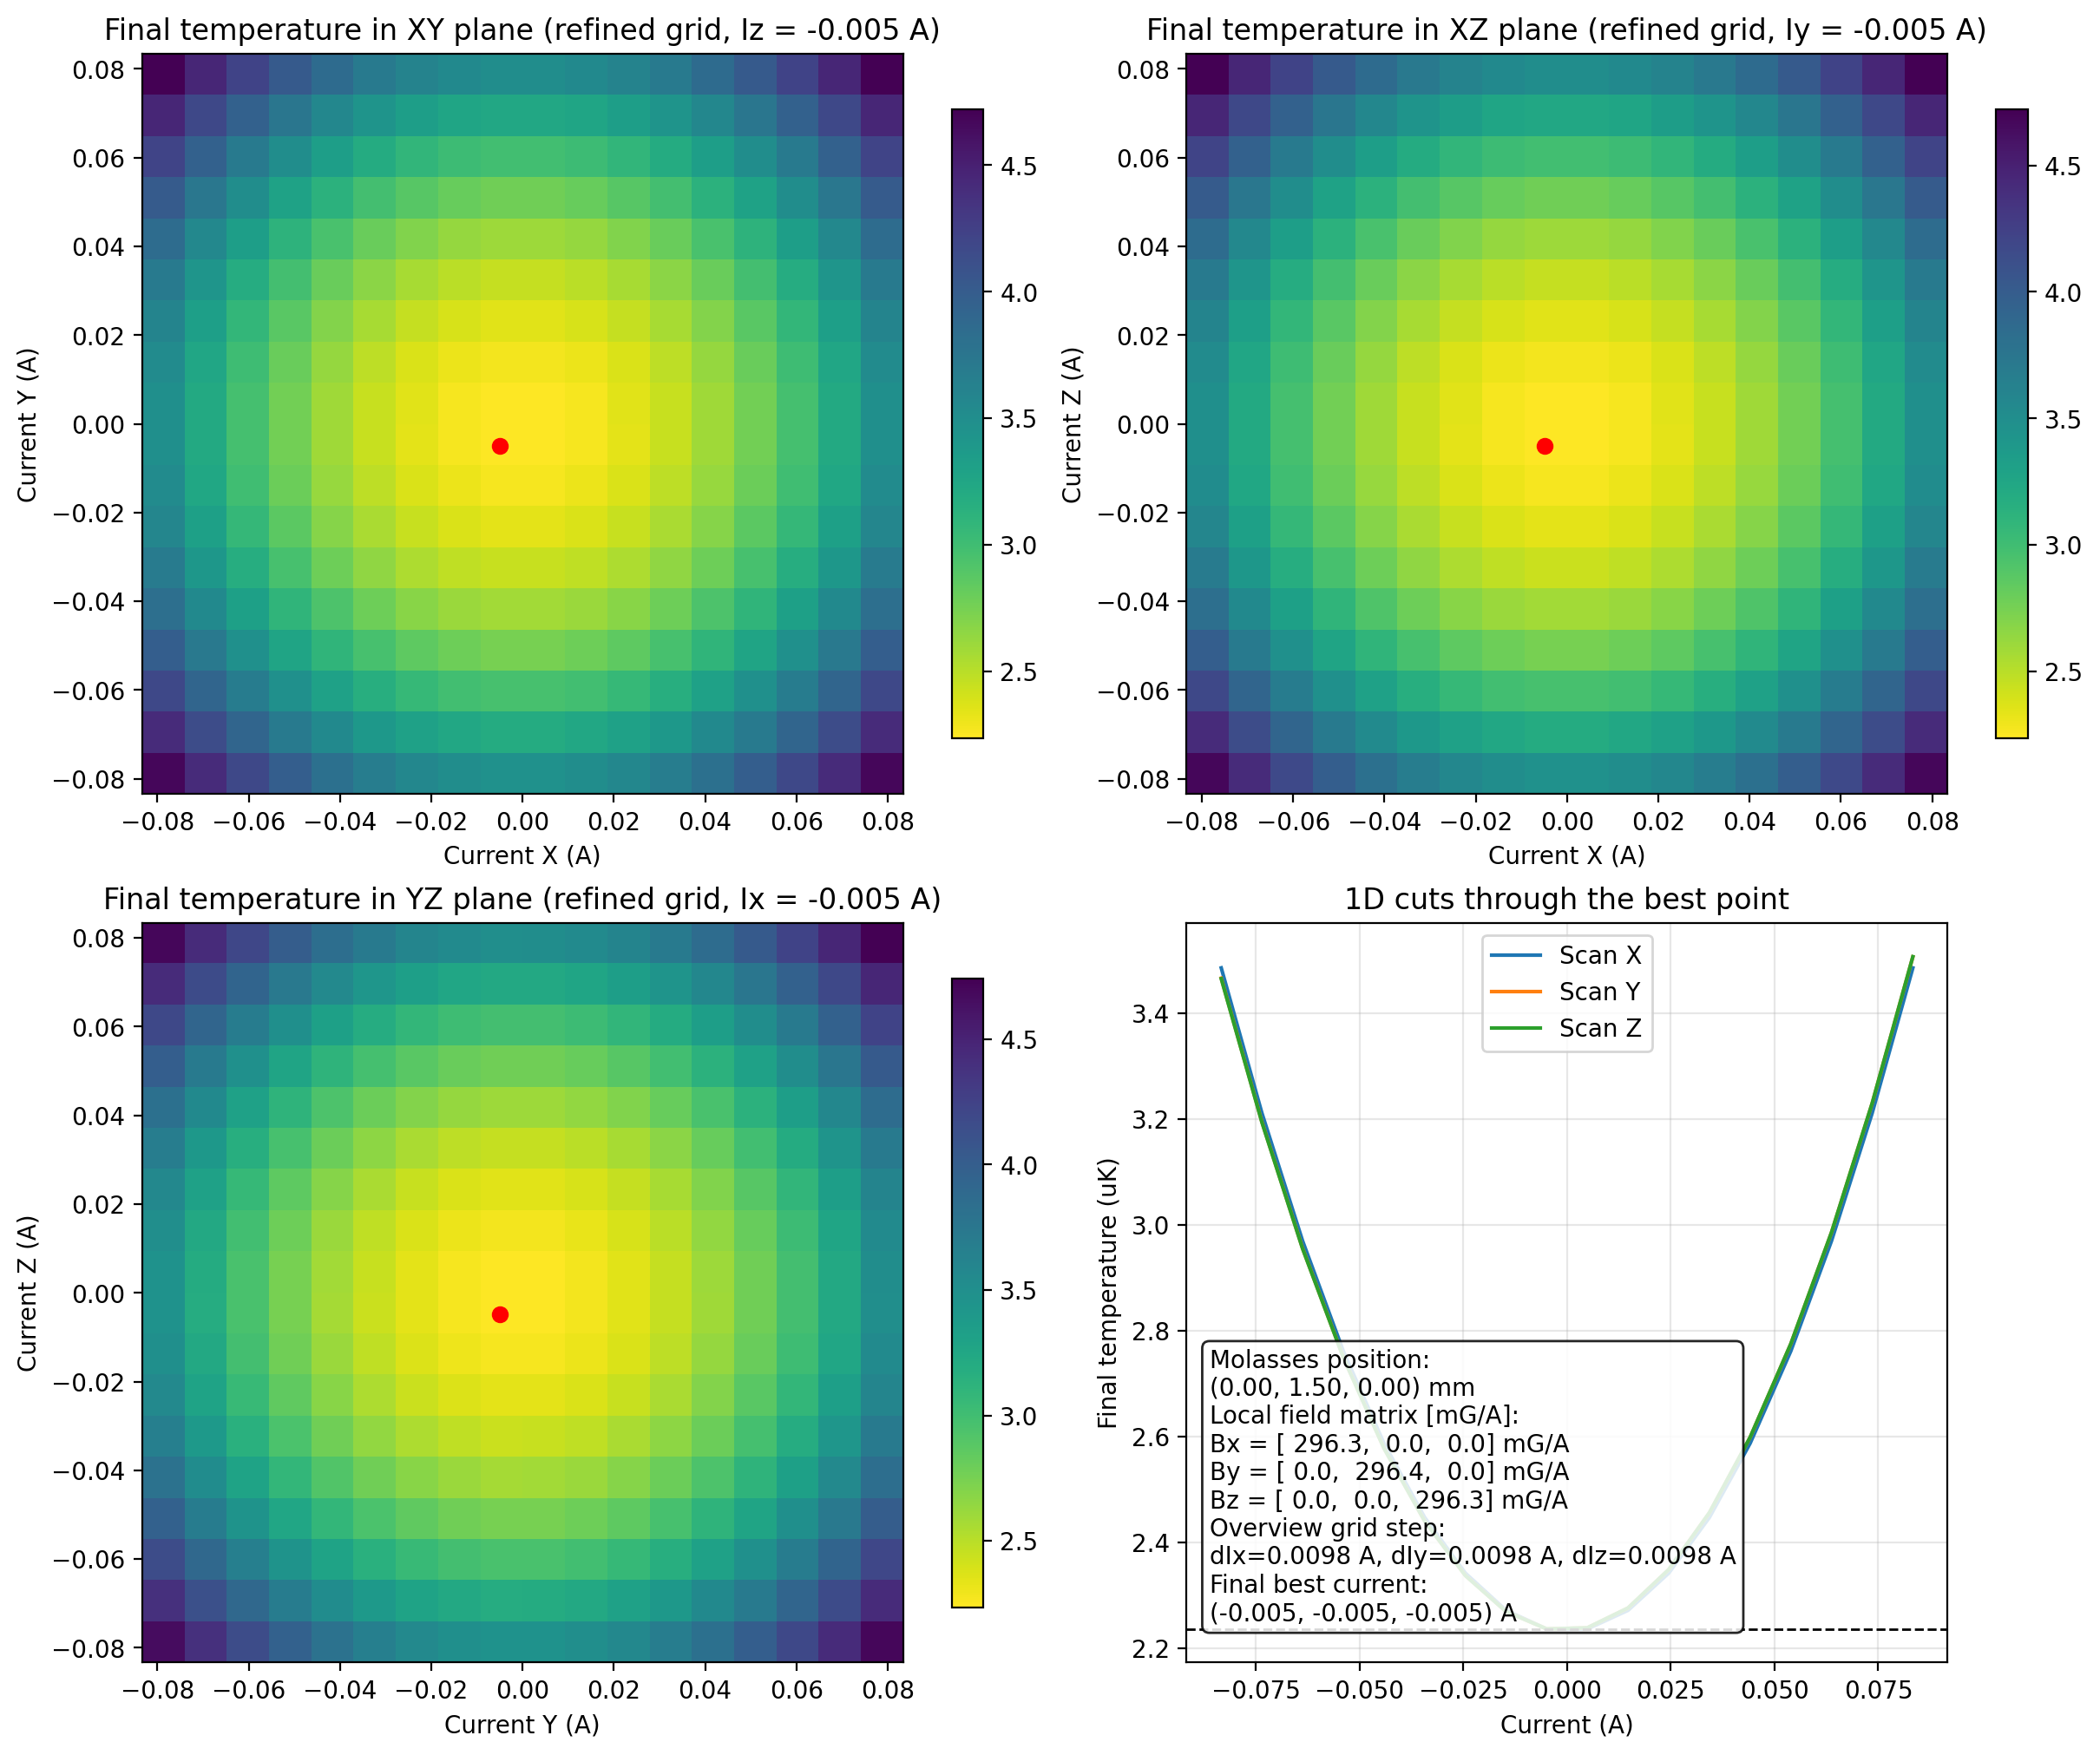
\includegraphics[width=0.92\textwidth]{rb87_pgc_current_scan_overview.png}
  \caption{Overview figure generated by the simulation. The three heat maps show final temperature on the $XY$, $XZ$, and $YZ$ current slices around the best point. The lower-right panel shows one-dimensional cuts through the optimum.}
  \label{fig:overview}
\end{figure}

Figure~\ref{fig:overview} is the main optimization view. It answers the practical question: ``Which compensation current triplet minimizes the final molasses temperature?'' The heat maps reveal the temperature landscape in current space, while the one-dimensional cuts clarify the curvature and width of the optimum.

\subsection{Time-Domain Dynamics Figure}

\begin{figure}[H]
  \centering
  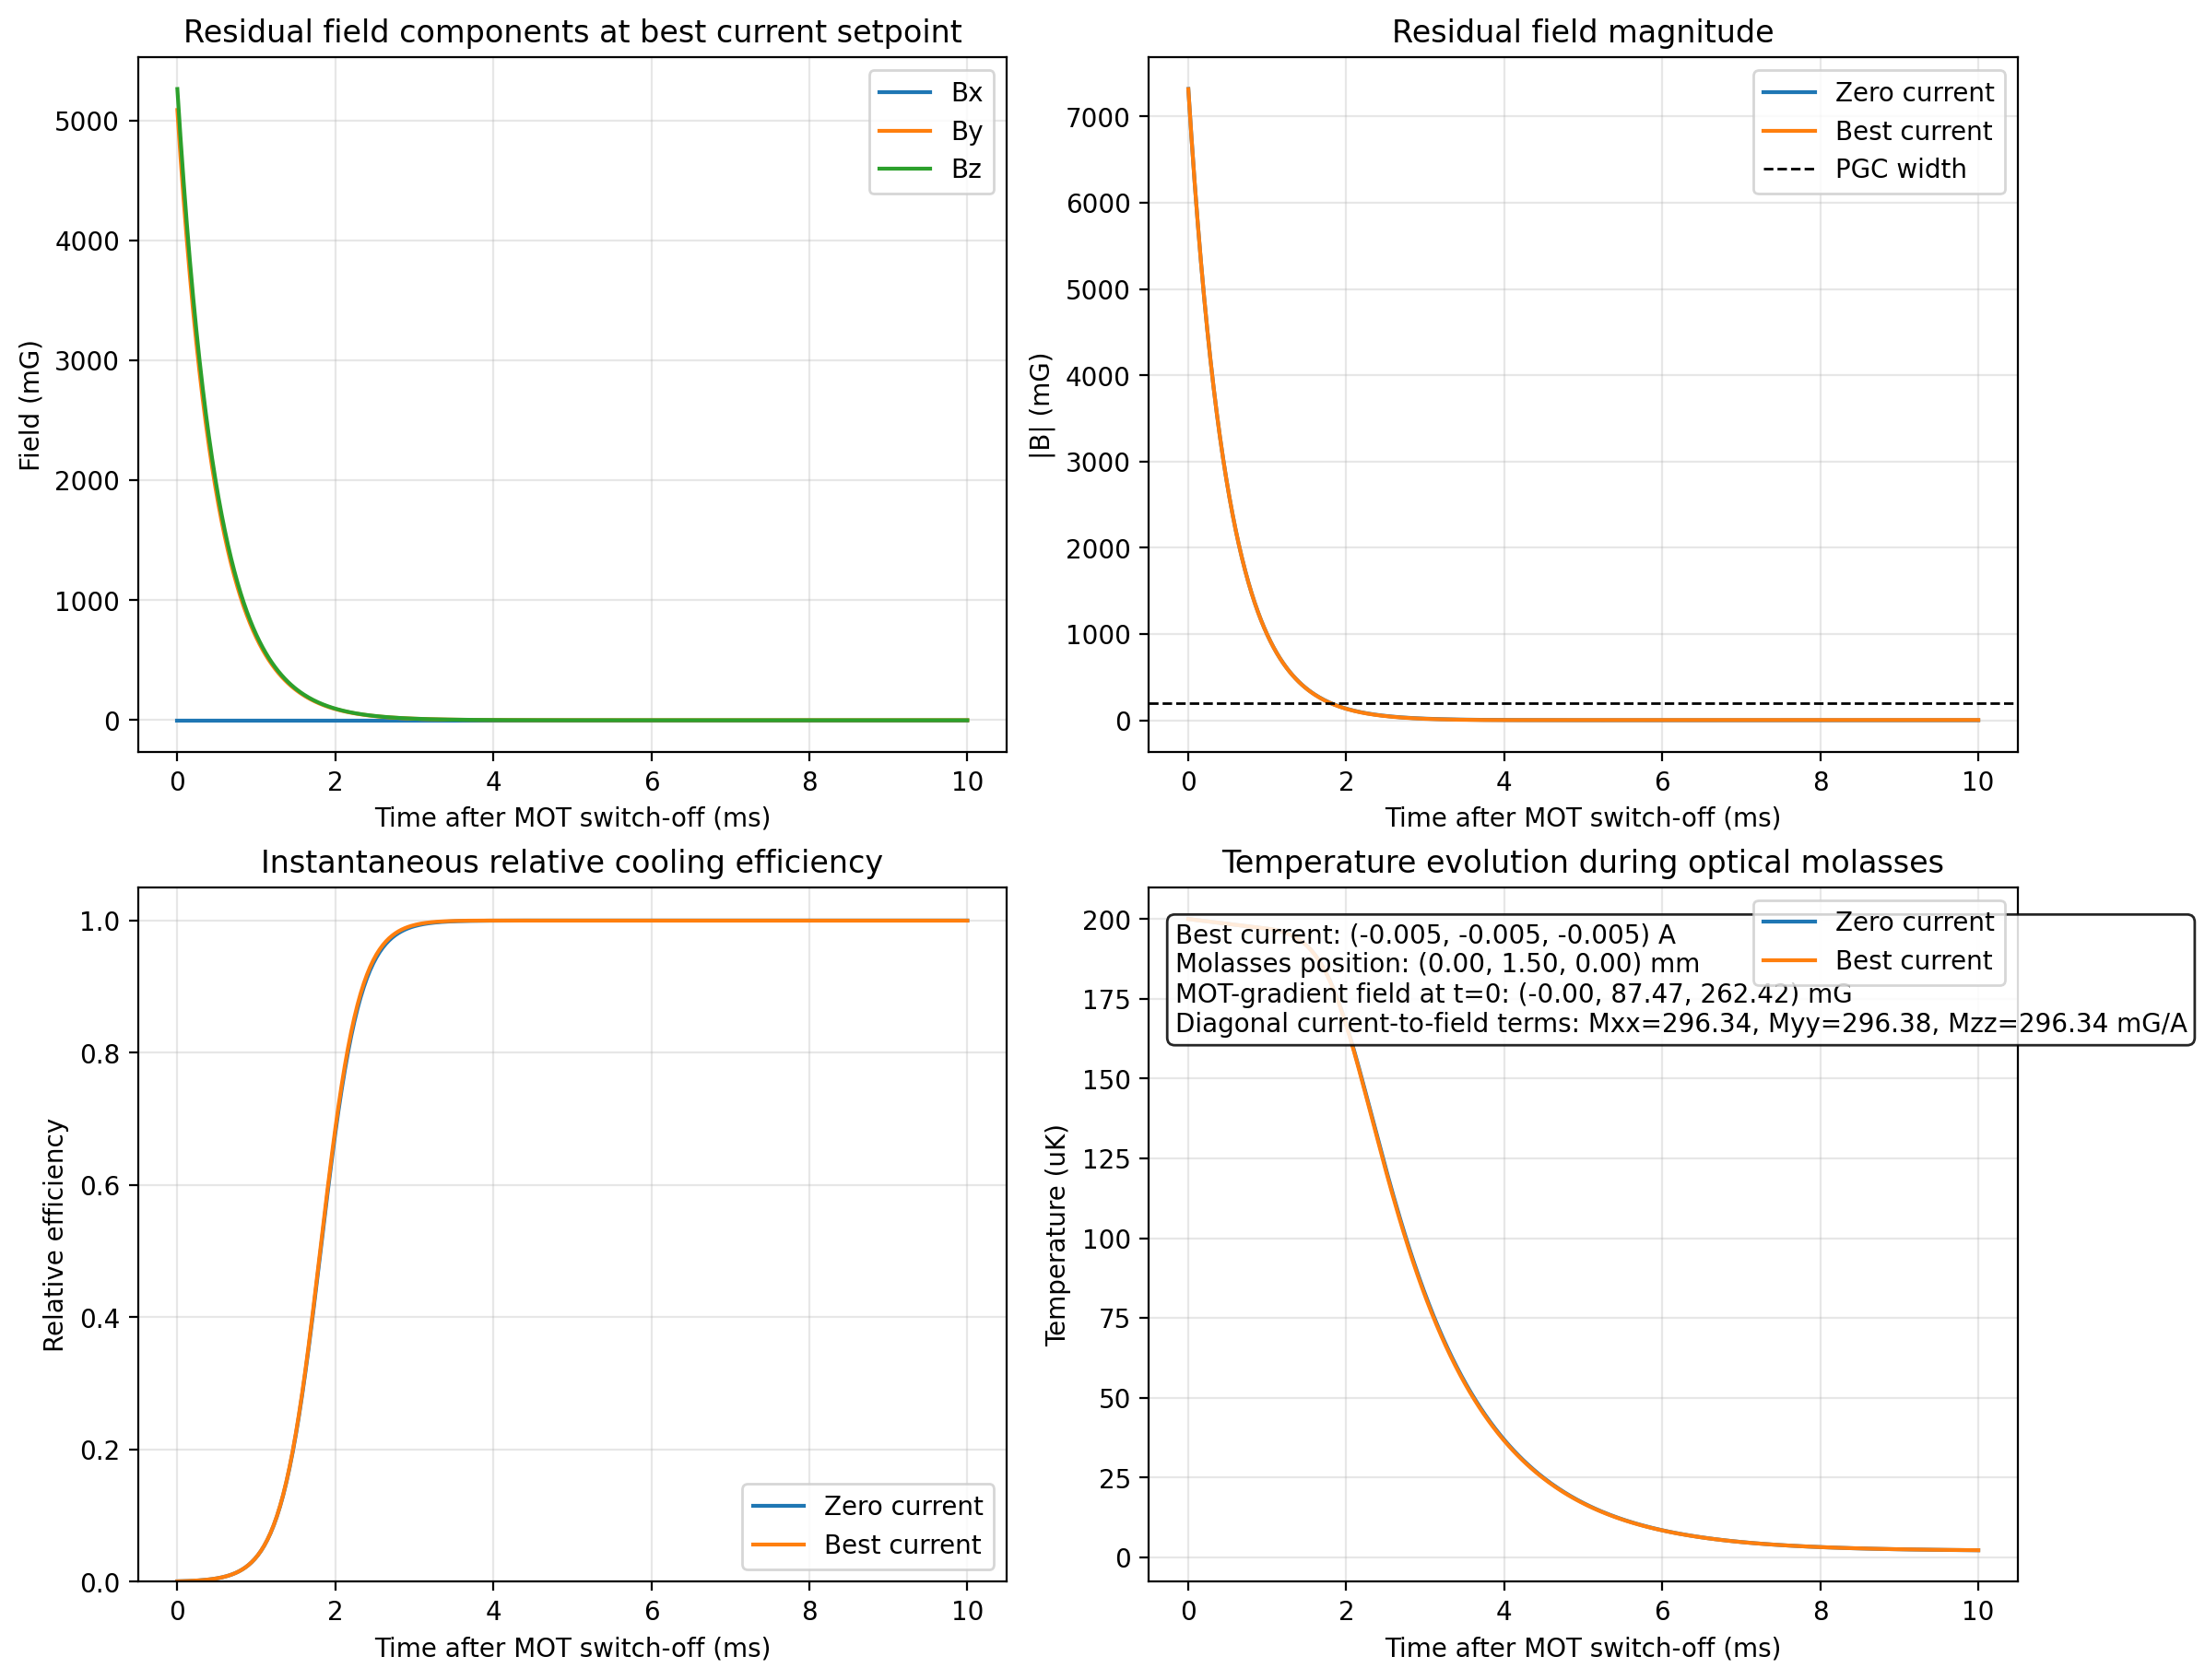
\includegraphics[width=0.92\textwidth]{rb87_pgc_current_scan_dynamics.png}
  \caption{Time-domain dynamics figure. The panels show the vector components of the residual field, the field magnitude, the relative cooling efficiency, and the temperature evolution during molasses.}
  \label{fig:dynamics}
\end{figure}

Figure~\ref{fig:dynamics} explains \emph{why} a given current triplet performs better than another one. It shows how the residual field decays after MOT switch-off, how that field maps into the cooling efficiency, and how the temperature approaches its field-dependent equilibrium value.

\subsection{Local Spatial Field Figure}

\begin{figure}[H]
  \centering
  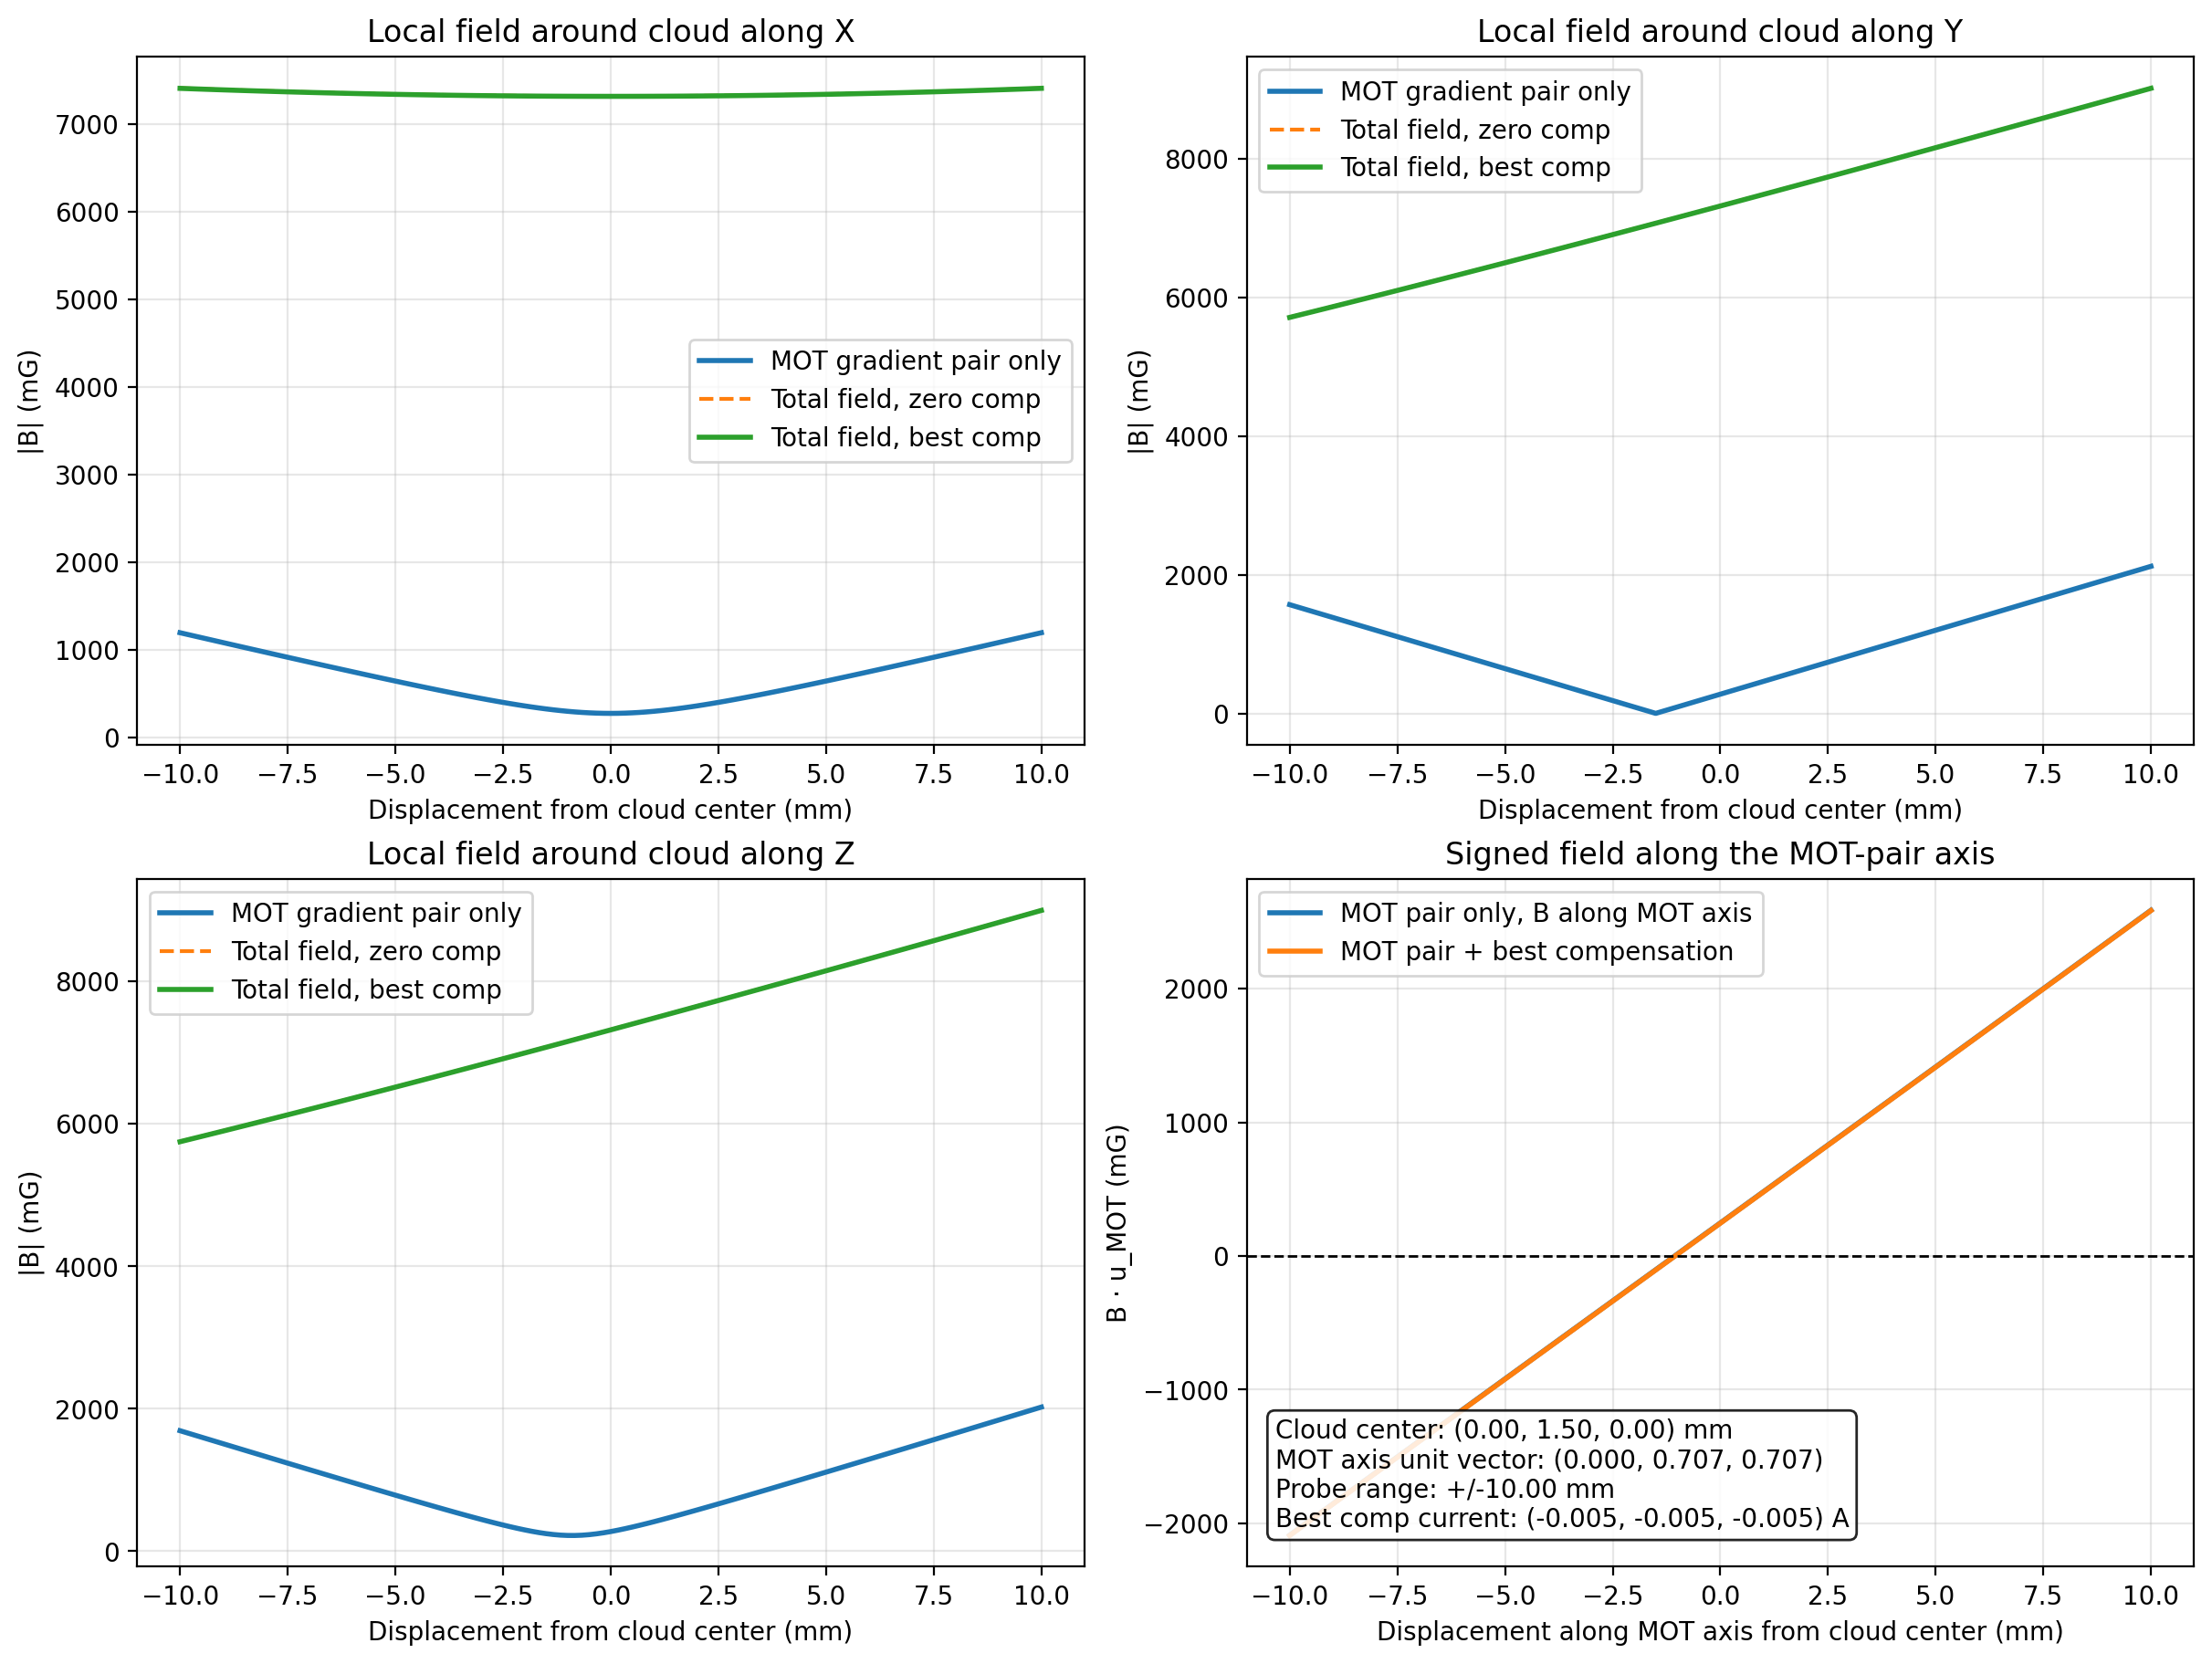
\includegraphics[width=0.92\textwidth]{rb87_pgc_current_scan_spatial_field.png}
  \caption{Local spatial magnetic-field figure. The first three panels show field-magnitude cuts around the cloud along $X$, $Y$, and $Z$. The fourth panel shows the signed field along the MOT-pair axis. The figure compares the MOT gradient pair alone, the uncompensated total field, and the total field at the best compensation current.}
  \label{fig:spatial}
\end{figure}

Figure~\ref{fig:spatial} is especially important once the cloud is displaced from the origin. It visualizes how the local quadrupole field from the 3D MOT coils changes across the cloud neighborhood and how much that profile is improved by the compensation coils. This figure is the clearest diagnostic of whether the compensation is only pointwise or whether it also improves the local field homogeneity.

\section{Configuration and Output Files}

Each simulation run typically produces:
\begin{itemize}
  \item \texttt{*\_scan.csv}: coarse scan table,
  \item \texttt{*\_refined\_scan.csv}: refined scan table,
  \item \texttt{*\_overview.png}: temperature maps in current space,
  \item \texttt{*\_dynamics.png}: time-domain residual-field and temperature curves,
  \item \texttt{*\_spatial\_field.png}: local spatial magnetic-field curves around the cloud,
  \item \texttt{*\_summary.txt}: summary of the best point and derived quantities,
  \item \texttt{*\_resolved\_config.json}: full input plus derived matrices and gradients.
\end{itemize}

The resolved configuration file stores, among other quantities:
\begin{itemize}
  \item the compensation current-to-field matrix at the chosen cloud position,
  \item the MOT residual field at the cloud position at $t=0$,
  \item the local MOT gradient Jacobian near the cloud center.
\end{itemize}

\section{Graphical User Interface}

The Qt and Tk interfaces provide:
\begin{itemize}
  \item editable molasses parameters,
  \item editable compensation-coil geometry and current-scan ranges,
  \item editable 3D MOT gradient-coil geometry and axis direction,
  \item editable local spatial-probe range,
  \item interactive overview, dynamics, and spatial-field plots,
  \item JSON configuration load/save,
  \item export and browsing of generated figures and data files.
\end{itemize}

\section{Model Scope and Limitations}

The current simulation has several strengths:
\begin{itemize}
  \item it has moved beyond a purely ideal center-point compensation model,
  \item it explicitly includes the residual effect of the 3D MOT quadrupole field when the cloud is displaced from the zero,
  \item it provides a local spatial-field diagnostic rather than only a single-point time trace.
\end{itemize}

However, several limitations should be kept in mind:
\begin{itemize}
  \item the temperature evolution still uses the field at the cloud center rather than a full spatial average over a finite cloud distribution,
  \item the switch-off behavior is modeled with a single exponential time constant,
  \item the PGC / Sisyphus cooling model is semi-empirical rather than derived from a full multilevel optical Bloch treatment.
\end{itemize}

\section{Possible Future Extensions}

To make the simulation closer to the experiment, the following extensions would be natural:
\begin{itemize}
  \item include a finite cloud size and perform three-dimensional spatial averaging,
  \item introduce a separate decay constant for the MOT gradient residual,
  \item include installation errors such as tilt, offset, and asymmetry of the compensation and MOT coils,
  \item fit the model parameters against measured temperature-versus-current data.
\end{itemize}

\section{Conclusion}

The physical logic of the code can be summarized in four steps:
\begin{enumerate}
  \item compute the local magnetic field produced by the compensation coils and the 3D MOT gradient coils,
  \item build the time-dependent total residual field during optical molasses,
  \item map that field into cooling efficiency, equilibrium temperature, and cooling time,
  \item perform a current scan with optional refinement to locate the best compensation point.
\end{enumerate}

In this sense, the code is useful both as an optimization tool for bias-coil currents and as a diagnostic tool for understanding why a displaced atomic cloud may suffer reduced cooling performance due to residual MOT-gradient fields.

\end{document}
